\begin{figure}[t]
\centering
\small
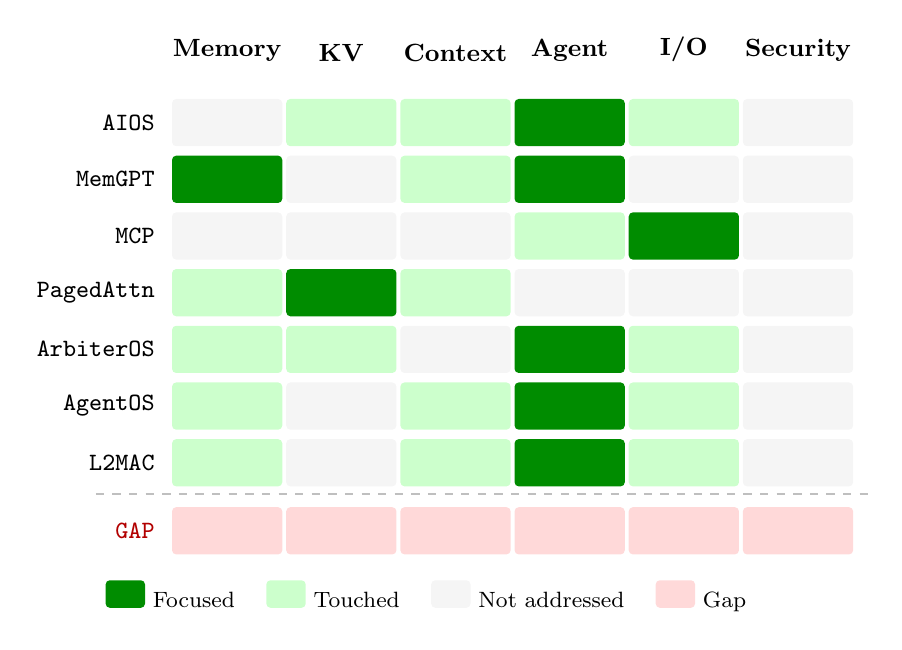
\begin{tikzpicture}[
    x=1.45cm, y=0.72cm,
    every node/.style={font=\small},
    focused/.style={fill=green!55!black, text=white, rounded corners=1.5pt, minimum width=1.4cm, minimum height=0.6cm, inner sep=0pt},
    touched/.style={fill=green!20, text=black, rounded corners=1.5pt, minimum width=1.4cm, minimum height=0.6cm, inner sep=0pt},
    notaddr/.style={fill=gray!8, text=gray!45, rounded corners=1.5pt, minimum width=1.4cm, minimum height=0.6cm, inner sep=0pt},
    gap/.style={fill=red!15, text=red!70!black, rounded corners=1.5pt, minimum width=1.4cm, minimum height=0.6cm, inner sep=0pt, font=\small\bfseries},
    rowlabel/.style={anchor=east, font=\small\ttfamily},
    collabel/.style={anchor=south, font=\small\bfseries, align=center, text width=1.5cm},
]

% Column labels (layers)
\node[collabel] at (1, 8.2) {Memory};
\node[collabel] at (2, 8.2) {KV};
\node[collabel] at (3, 8.2) {Context};
\node[collabel] at (4, 8.2) {Agent};
\node[collabel] at (5, 8.2) {I/O};
\node[collabel] at (6, 8.2) {Security};

% Row labels (works) and cells
% Row 1: AIOS
\node[rowlabel] at (0.45, 7.3) {AIOS};
\node[notaddr]   at (1, 7.3) {};
\node[touched]   at (2, 7.3) {~};
\node[touched]   at (3, 7.3) {~};
\node[focused]   at (4, 7.3) {~};
\node[touched]   at (5, 7.3) {~};
\node[notaddr]   at (6, 7.3) {};

% Row 2: MemGPT
\node[rowlabel] at (0.45, 6.3) {MemGPT};
\node[focused]   at (1, 6.3) {~};
\node[notaddr]   at (2, 6.3) {};
\node[touched]   at (3, 6.3) {~};
\node[focused]   at (4, 6.3) {~};
\node[notaddr]   at (5, 6.3) {};
\node[notaddr]   at (6, 6.3) {};

% Row 3: MCP
\node[rowlabel] at (0.45, 5.3) {MCP};
\node[notaddr]   at (1, 5.3) {};
\node[notaddr]   at (2, 5.3) {};
\node[notaddr]   at (3, 5.3) {};
\node[touched]   at (4, 5.3) {~};
\node[focused]   at (5, 5.3) {~};
\node[notaddr]   at (6, 5.3) {};

% Row 4: PagedAttention
\node[rowlabel] at (0.45, 4.3) {PagedAttn};
\node[touched]   at (1, 4.3) {~};
\node[focused]   at (2, 4.3) {~};
\node[touched]   at (3, 4.3) {~};
\node[notaddr]   at (4, 4.3) {};
\node[notaddr]   at (5, 4.3) {};
\node[notaddr]   at (6, 4.3) {};

% Row 5: ArbiterOS
\node[rowlabel] at (0.45, 3.3) {ArbiterOS};
\node[touched]   at (1, 3.3) {~};
\node[touched]   at (2, 3.3) {~};
\node[notaddr]   at (3, 3.3) {};
\node[focused]   at (4, 3.3) {~};
\node[touched]   at (5, 3.3) {~};
\node[notaddr]   at (6, 3.3) {};

% Row 6: AgentOS
\node[rowlabel] at (0.45, 2.3) {AgentOS};
\node[touched]   at (1, 2.3) {~};
\node[notaddr]   at (2, 2.3) {};
\node[touched]   at (3, 2.3) {~};
\node[focused]   at (4, 2.3) {~};
\node[touched]   at (5, 2.3) {~};
\node[notaddr]   at (6, 2.3) {};

% Row 7: L2MAC
\node[rowlabel] at (0.45, 1.3) {L2MAC};
\node[touched]   at (1, 1.3) {~};
\node[notaddr]   at (2, 1.3) {};
\node[touched]   at (3, 1.3) {~};
\node[focused]   at (4, 1.3) {~};
\node[touched]   at (5, 1.3) {~};
\node[notaddr]   at (6, 1.3) {};

% Separator line
\draw[gray!50, dashed, thick] (-0.15, 0.75) -- (6.65, 0.75);

% Row 8: GAP
\node[rowlabel, font=\small\ttfamily\bfseries, text=red!70!black] at (0.45, 0.1) {GAP};
\node[gap]   at (1, 0.1) {~};
\node[gap]   at (2, 0.1) {~};
\node[gap]   at (3, 0.1) {~};
\node[gap]   at (4, 0.1) {~};
\node[gap]   at (5, 0.1) {~};
\node[gap]   at (6, 0.1) {~};

% Legend
\node[anchor=north west, font=\footnotesize] at (-0.15, -0.6) {%
    \tikz\node[focused, minimum width=0.5cm, minimum height=0.35cm]{}; Focused \quad
    \tikz\node[touched, minimum width=0.5cm, minimum height=0.35cm]{}; Touched \quad
    \tikz\node[notaddr, minimum width=0.5cm, minimum height=0.35cm]{}; Not addressed \quad
    \tikz\node[gap, minimum width=0.5cm, minimum height=0.35cm]{}; Gap
};

\end{tikzpicture}
\caption{Coverage of system layers by existing works}
\label{fig_coverage_map}
\end{figure}
